\subsection{Addressing modes}

In order to keep complexity of an implementation low, only simple addressing is included in the \ac{isa}. \autoref{fig:addressing_modes_implemented} shows the same hierarchy of addressing modes as \autoref{fig:addressing_modes_general} but highlights the ones used by \ac{ava}.

\begin{figure}[h!]
    \centering
    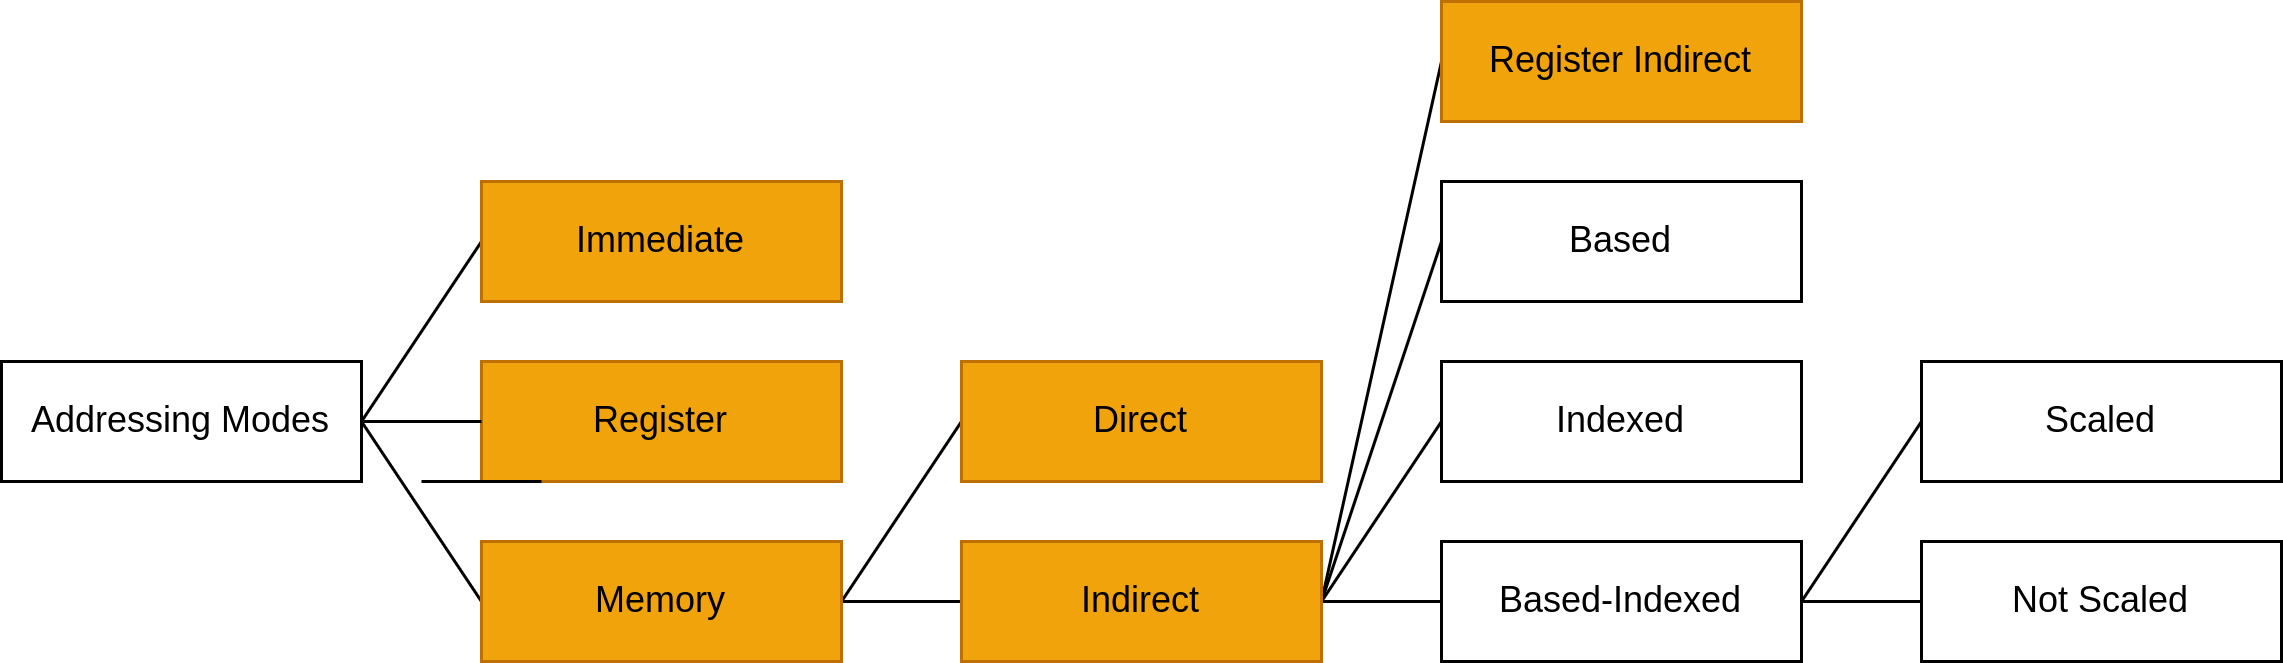
\includegraphics[width=0.7\textwidth]{images/drawio/addressing_modes_implemented.png}  % Replace with your image file
    \caption{Hierarchical overview of addressing modes with implemented modes highlighted. (Modified from S. Dandamudi, laid out horizontally and compacted for readability \cite{sivarama_addrmodes})}
    \label{fig:addressing_modes_implemented}
\end{figure}

All of these addressing modes share the property of containing no arithmetic for calculating an address. This means that an implementation only needs to route connections between components without additional components required for computation. Since the more complex addressing modes are used for implementing high level constructs in a performant manner, they can be substituted with multiple primitive operations. The programmer must calculate offsets for members of a piece of structured data explicitly using arithmetic instructions.
